% ARR version: compile main.tex (anonymous, line numbers).
% arXiv version: compile arxiv.tex, which defines \arxivversion and inputs this file.
\documentclass[11pt]{article}
\ifdefined\arxivversion
\usepackage[final]{acl}
\else
\usepackage[review]{acl}
\fi
\usepackage{times}
\usepackage{latexsym}
\usepackage{amsmath,amssymb}
\usepackage{booktabs}
\usepackage{graphicx}
\usepackage{microtype}
\usepackage{inconsolata}
\usepackage{xcolor}

\title{How Many Documents Cover a Corpus}

\ifdefined\arxivversion
\author{Mao Li \\
  University of Michigan \\
  \texttt{maolee@umich.edu}}
\else
\author{Anonymous ACL submission}
\fi

\begin{document}
\maketitle

\begin{abstract}
If we read 15 documents from a corpus, how much of the corpus have we seen? Researchers who study text read samples because they cannot analyze every document. A survey sample comes with a formula for its size and a margin of error, and a sample of text comes with neither. We measure what a sample has missed as the percentage of the corpus with no document of the same content in the sample. A text encoder turns each document into an embedding, a list of numbers, so that documents with similar meaning have embeddings close together. Two documents count as the same content when their embeddings lie closer than a distance the researcher chooses, and two large language models judged pairs of documents to tell which distance means the same specific content and which means the same topic. We estimate the missed percentage from the sample alone with a classical estimator built on what we call the isolation rate, the percentage of sampled documents with no other sampled document of the same content. The main lesson is that a random sample is a poor use of a reading budget on corpora that repeat themselves, in which many documents make the same claim. With the whole corpus embedded, a researcher can divide it into as many groups of similar documents as the budget allows. The documents nearest the centres of these groups cover far more of such a corpus than the same number of random documents. At the level of topics, 15 documents chosen this way often miss about half as much of the corpus as 15 random documents. On corpora whose documents rarely share specific content, no choice of documents helps at the level of specific content, because a document unlike every other is covered only by reading it. The isolation rate of a random pilot of 100 documents tells a researcher in advance which of the two cases applies. To plan the size of a sample, we show that on most corpora we tested a larger sample and a looser definition of the same content trade against each other at a fixed rate. The rate is set by the intrinsic dimension of the corpus, the number of independent ways in which its documents differ in meaning. This rate gives a sample size formula. In 77 of 83 tests, each a combination of corpus, target and distance, the sample actually needed fell between two thirds and one and a half times the formula's answer. A larger pilot of 2{,}000 documents shows in advance whether the formula can be trusted for a given corpus.
\end{abstract}

\section{Introduction}

Researchers who study large collections of text rarely read all of them. An annotation team codes a few thousand posts out of millions, a large language model summarizes a few hundred documents because the whole corpus does not fit in its context window, and a qualitative researcher keeps reading until further documents stop adding codes. Each of these practices assumes that the documents in hand stand for the documents left unread. Yet the number of documents is usually set by budget or by feel. If we read 15 posts from a corpus of 10{,}000, a number a person can read in a few minutes, have we understood the corpus? If not, would 100 posts be enough, or 1{,}000?

Survey research has a settled answer to the same question for a human population. The researcher states how much people differ on the quantity of interest (the population variance $\sigma^{2}$) and how large an error is tolerable ($e$), and the formula $n = z^{2}\sigma^{2}/e^{2}$ gives the number of people to interview \citep{cochran1977, kish1965}. Every estimate from the sample then carries a margin of error. A sample of a corpus comes with neither a sample size formula nor a margin of error. This paper builds both for the question a reader of a sample usually has in mind: how much of the corpus has a document like it among the documents we read?

The answer depends on what counts as alike. Two posts can be about the same topic, such as the 2020 United States Census, while making different claims, and two other posts can repeat the same claim in different words. We place each document in an embedding space, where a text encoder puts documents with similar meaning close together, and we measure how alike two documents are by the cosine distance between them. The user then chooses a distance $r$ below which two documents count as the same content. To give $r$ a concrete meaning, we asked two large language models, Qwen3.8 and Gemma~4, to judge about 4{,}000 pairs of documents at a range of distances. For each corpus we found the distance below which most pairs are about the same specific claim, question, event or story, and the larger distance below which most pairs share at least a topic (Section~\ref{sec:rcal}).

At these two distances the question of the 15 posts has a clear answer, and it differs from corpus to corpus (Table~\ref{tab:reader}). Take the 17{,}202 tweets about the 2020 Census that contain the word ``illegal''. In a random sample of 15 of them, 98\% of the corpus has a tweet on the same topic, so a reader of those 15 tweets has seen nearly every topic the corpus discusses. Only 38\% of the corpus, however, has a tweet in the sample that makes the same specific point. Now take 10{,}000 personal stories from the TIFU forum on Reddit, in which users tell how they messed something up. In a sample of 15 stories, only 1.5\% of the corpus has a story on the same topic. Even in a sample of 1{,}000 stories, only 10\% of the corpus has a story about the same event. Whether a sample is enough therefore depends on the corpus and on what the reader needs to know.

The share of a corpus that has no document like it in the sample is called the missing mass, and statistics has a classical way to estimate it without looking at the unread documents. During the Second World War, I.~J. Good and Alan Turing noticed that a sample reveals how much it is missing through the items it contains only once \citep{good1953}. If most words in a sample of text occur once, many more words remain unseen. If every word in the sample has occurred several times, few words remain. \citet{maurer2022missing} carried this idea from categories to distances. His estimator $G$, which we call the isolation rate, is the share of documents in the sample that have no other sampled document within $r$, that is, the share of the documents we read that were unlike anything else we read. For example, in a sample of 15 of the Census tweets with ``illegal'', 64\% of the tweets have no close match among the other 14. This is the estimate. The truth, which we can compute because we have the whole corpus, is that 62\% of the corpus has no close match in the sample. A reader can therefore learn how much a sample has missed from the sample alone. Maurer's paper is theoretical. It proves how far $G$ can be from the missing mass, and it leaves open how $G$ falls as the sample grows, which is what a researcher needs in order to plan a sample. To our knowledge the estimator has not yet been used on text.

How $G$ falls with the sample size follows from a classical result about the distances between random points \citep{levina2005, facco2017twonn, penrose2003rgg}. Suppose the documents of a corpus differ from one another along $d$ independent directions of meaning, where $d$ is called the intrinsic dimension of the embedded corpus and can be estimated from the distances between documents. Then the chance that a document has no neighbour within $r$ among $n$ sampled documents depends on $n$ and $r$ only through the product $n r^{d}$. In other words, a larger sample and a looser definition of the same content can stand in for each other, at a rate set by $d$. The product has a direct meaning for sampling. When the definition of the same content becomes twice as strict, that is, when $r$ is halved, the number of documents close enough to count as a match shrinks $2^{d}$ times, so the sample must grow $2^{d}$ times to cover the corpus as well as before. For the medical questions of the AskDocs forum and the TIFU stories, $d$ is about 13, so a definition twice as strict requires about 8{,}000 times as many documents. The intrinsic dimension thus does for a corpus what the variance does for a survey population. It is the property that sets how large a sample must be.

We test this law on seventeen pairs of corpus and encoder, which include medical questions, personal stories, election discussion, tweets about the 2020 Census, posts from Truth Social and Bluesky, and synthetic data with a known answer. The law holds on most of these corpora, it needs one correction for finite corpora, and it fails on a recognizable kind of corpus.

\begin{enumerate}
\item On ten of the seventeen pairs, $G$ depends on the sample size and the distance only through $n r^{d}$. The law has two constants besides $d$, and a fit of these constants on samples of up to 1{,}000 documents predicts $G$ for samples seven times larger. Solved for $n$, the law gives the sample size that brings $G$ down to a target, such as 20\% of the sampled documents isolated. We tested this formula in 83 cases, one for each combination of corpus, target and distance at which the true answer lay beyond 1{,}000 documents. In 77 of the 83 cases, the sample that actually reached the target held between two thirds of the formula's number and one and a half times that number. A formula answer of 1{,}500 documents thus meant an actual need between 1{,}000 and 2{,}250. The standard tool from ecology for the same task, the extrapolation of \citet{chao2012coverage}, predicts $G$ for a sample twice as large with an average error two to nine times that of the law.
\item For a corpus of $N$ documents, the missing mass is $G\,(1 - n/N)$. The correction is needed because $G$ describes the documents a sample has not reached, and the $n$ sampled documents are reached by definition. Survey sampling knows the same factor as the finite population correction. With it, the estimate is on average one percentage point from the true missing mass.
\item The law fails on the other seven pairs. Five are political corpora, among them a forum in which short slogans repeated many times sit beside longer discussion. One is a second encoding of that forum, and one is a synthetic mixture of topics. A test run on a pilot sample of 2{,}000 documents separates the seven failing pairs from the ten passing pairs before the full sample is drawn.
\end{enumerate}

Taken together, these results let a researcher size a sample before reading it. We set a modest target, that half of the corpus should have a document with the same specific content in the sample. On corpora that repeat a few claims, such as Census tweets selected by a keyword or a forum about one election, a few hundred posts reach this target. On forum questions, personal stories and the Truth Social posts, the sample must hold more than 40\% of the corpus. The reference point is a corpus in which no two documents share content. There the sample matches only itself, so reaching the target takes exactly half of the corpus, and the forum questions, stories and Truth Social posts come close to this limit. Two pilots of different sizes serve two purposes. A pilot of 100 documents already tells which kind of corpus a researcher has, since in it no document has a match on the corpora that come close to the limit. A pilot of 2{,}000 documents is needed to fit the law and predict the required sample.

\section{Background}

\subsection{Sample coverage in the discrete case}

A sample of $n$ draws from a population of categories covers the categories it has seen. The mass it has missed is the total probability of the unseen categories. Let $f_k$ be the number of categories that appeared exactly $k$ times in the sample. \citet{good1953} showed that $f_1/n$, the share of draws whose category appeared once, estimates the missing mass with small bias. Ecologists took the estimator as the basis of a sampling theory for species. \citet{chao1984} bounded the number of unseen species from $f_1$ and $f_2$, and \citet{chao2012coverage} wrote the expected coverage of a sample enlarged by $m$ draws as a closed form in $n$, $f_1$ and $f_2$, so that a survey of a habitat can be stopped at a target coverage. \citet{efron1976} asked how many words Shakespeare knew with the same machinery, and \citet{orlitsky2016unseen} gave the optimal prediction of the number of unseen species for a sample up to about $n \log n$ times larger than the one in hand.

The estimators have reached text and machine learning a few times. \citet{hajic2025} apply the Chao bound to a catalogue of chant to say how far a collection is from complete. \citet{tran2017} fit species models to the answers to an open ended survey question to predict when new answers stop appearing. \citet{chung2018unknown} count the unknown examples of a training set with the same estimator, a species being a unique example, and \citet{pal2026blindspot} estimate the mass of deployment states a classifier has never seen. In all four a species is a discrete label and two items either match or do not.

\subsection{The missing mass in a metric space}

\citet{maurer2022missing} removed the discreteness. In a metric space with distance $d(\cdot, \cdot)$, the missing mass of a sample $X_1, \dots, X_n$ at scale $r$ is the probability that a new draw lies farther than $r$ from every $X_i$. Maurer calls it the conditional missing mass because it is conditional on the sample drawn. His estimator is
\begin{equation}
G(X, r) = \frac{1}{n}\,\big|\{k : d(X_k, X_i) > r \text{ for all } i \neq k\}\big| ,
\label{eq:G}
\end{equation}
the share of sample points with no other sample point within $r$. In the discrete case, with $d(x, y) = 1$ for $x \neq y$ and $r < 1$, it is $f_1/n$. Maurer proved that $G$ exceeds the conditional missing mass by at most $1/n$ in expectation and that the variance of $G$ minus the conditional missing mass is at most $3/n$ (his Theorem 2.1). The paper is theory. It sketches anomaly detection and coding as applications, and it contains no data, no embeddings and no statement about how $G$ falls with $n$. That dependence is the subject of the nearest neighbour distance law: for a density $f$ on a set of dimension $d$, the probability that a point has no neighbour within $r$ among $n$ others is close to $\exp(-n f(x)\, v_d\, r^{d})$, with $v_d$ the volume of the unit ball \citep{evans2002, penrose2003rgg}. The same law underlies the correlation dimension of \citet{grassberger1983} and the estimators of \citet{levina2005} and \citet{facco2017twonn}. The nearest ecological construction is the attribute diversity of \citet{chao2019attribute}, in which two species closer than a threshold $\tau$ count as partly the same and diversity is reported as a function of $\tau$. We treat $r$ the same way, as a resolution the user chooses.

\subsection{Diversity of a sample in embedding space}

Several measures describe how spread out a set of embedded points is. The Vendi score is the exponential of the entropy of the eigenvalues of the sample's cosine kernel matrix, an effective number of distinct items \citep{friedman2023vendi}, and its cousins extend it to the orders of a Hill number \citep{pasarkar2024cousins}. The precision and recall of \citet{kynkaanniemi2019} count generated points inside nearest neighbour balls around a reference set, the density and coverage metrics of \citet{naeem2020} make those counts robust to the reference set's own spread, and MAUVE compares two distributions on a quantized embedding space \citep{pillutla2021mauve}. Each describes the sample in hand or compares two samples. None asks what a larger sample would cover, and none has a parameter in the role of a population variance. Core-set selection chooses points to minimise the largest distance from any point to the chosen set \citep{sener2018coreset}, and semantic deduplication removes points within a small distance of another \citep{abbas2023semdedup, lee2022dedup}. Both need the full embedded corpus, and neither says how many points a target needs. The intrinsic dimension of learned representations has been measured for images \citep{pope2021intrinsic}, for the layers of deep networks \citep{ansuini2019} and for text, where it separates human from generated writing \citep{tulchinskii2023}. We use it as the corpus parameter that sets a sample size.

\subsection{Saturation in practice}

Where a sample size for text is set at all, it is set by a stopping rule. Qualitative researchers stop interviewing when new interviews add no new code. \citet{guest2006} found that point at twelve interviews, and a review of 23 empirical tests by \citet{hennink2022} puts it at 9 to 17. \citet{depaoli2024} carry the rule to coding by a language model and track the slope of the count of unique codes. TopicGPT reports that its topic count levels off after about 600 documents and stops when 200 documents add no topic \citep{pham2024topicgpt}. \citet{maeda2025} fit an LDA model with eight topics to 522 open ended survey responses and find that a sample of 100 responses recovers over 60\% of the topics found on the full corpus and 250 recover about 70\%. These are observations of a coverage curve. The present paper gives the curve a parameter, the intrinsic dimension $d$, and an estimator.

\section{Method}

\subsection{Setting and estimand}

A corpus is a finite set of $N$ documents. Each is embedded by a fixed encoder and normalised, and the distance between two documents is the cosine distance of their embeddings. A sample is $n$ documents drawn without replacement. The user chooses a resolution $r$: two documents within $r$ of each other count as the same content for the purpose at hand. The quantity to estimate is the missing mass at resolution $r$,
\begin{equation}
M(n, r) = \frac{1}{N}\,\big|\{j : d(x_j, x_i) > r \text{ for all sampled } i\}\big| ,
\end{equation}
the share of corpus documents with no sampled document within $r$. Coverage is $1 - M$. The estimator is Maurer's $G$ of Equation~\ref{eq:G}, computed on the sample alone from each sampled document's distance to its nearest sampled neighbour.

The estimand is the finite corpus in hand. Sampling exists because the corpus is too large to annotate or to place in a model's context, and the full corpus is available to check the estimate. This is the setting of the experiments below, and it is what makes a finite population correction necessary.

\subsection{The collapse law}

Suppose the embedded documents lie near a manifold of intrinsic dimension $d$ with a smooth density. The mass of a ball of radius $r$ around a document is then of order $r^{d}$, and the probability that none of $n$ sampled documents falls in it is of order $\exp(-c\,n\,r^{d})$. Averaged over documents, the isolation rate $G$ should then depend on $n$ and $r$ only through the product $n r^{d}$. A density that varies across the manifold turns the single exponential into an average of exponentials with different rates, which is slower than exponential and well described by a stretched exponential. We therefore fit
\begin{equation}
\log\big(-\log G(n, r)\big) = a + b \log\big(n\,r^{d}\big),
\label{eq:collapse}
\end{equation}
with $d$ estimated beforehand and $a$ and $b$ fitted by least squares over the cells of an $(n, r)$ grid with $0.02 < G < 0.98$. An exponent $b = 1$ is the pure exponential, and $b < 1$ is the stretched form.

The dimension $d$ comes from the TwoNN estimator of \citet{facco2017twonn}, which uses only the ratio of each point's second to first nearest neighbour distance, on a pilot of 2{,}000 documents. We also fit Equation~\ref{eq:collapse} with $\log n$ and $\log r$ as separate regressors. The ratio of the $\log r$ coefficient to the $\log n$ coefficient is then an estimate of $d$ that owes nothing to TwoNN, and agreement between the two is a check on the law.

Solving Equation~\ref{eq:collapse} for $n$ gives the sample size at which the isolation rate at resolution $r$ reaches a target $\varepsilon$,
\begin{equation}
n^{*}(\varepsilon, r) = \left(\frac{\log(1/\varepsilon)}{e^{a}\, r^{d}}\right)^{1/b} .
\label{eq:nstar}
\end{equation}
This is the corpus analogue of $n = z^{2}\sigma^{2}/e^{2}$. The target $\varepsilon$ plays the part of the tolerated error, the resolution $r$ is set by the question, and $d$ is the property of the corpus that the formula needs, in the role of the variance. Each halving of $r$ multiplies $n^{*}$ by $2^{d/b}$.

\subsection{Finite population correction}

$G$ estimates the missing mass of the distribution that generated the corpus. When the estimand is the corpus itself, each sampled document is covered at distance zero, so the finite corpus's missing mass is smaller by the share of the corpus that was sampled. The corrected estimator is
\begin{equation}
\hat M(n, r) = G(n, r)\,\big(1 - n/N\big),
\label{eq:fpc}
\end{equation}
with $1 - n/N$ the finite population correction of survey sampling. The correction is negligible at $n \ll N$ and halves the estimate at $n = N/2$.

\subsection{A diagnostic for corpora with more than one scale}

Equation~\ref{eq:collapse} assumes one dimension for the whole corpus. The $R^2$ of the fit, and its $R^2$ on cells with larger $n$ than those used to fit, say whether the assumption holds. When it fails, two probes locate the cause: the share of documents with a near duplicate (a nearest neighbour within cosine distance 0.02), and the spread of TwoNN dimension across the corpus's $k$-means clusters.

\subsection{Theme coverage as a question about a partition}

A different question is how many documents are needed to see every theme. Once themes are a partition of the corpus with masses $m_1, \dots, m_K$, the expected mass of themes present in a sample of $n$ draws is
\begin{equation}
C_K(n) = \sum_{k=1}^{K} m_k\,\big(1 - (1 - m_k)^{n}\big),
\label{eq:gt}
\end{equation}
the Good-Turing expectation, and it depends on the corpus only through the masses. We test this with inventories of $K = 30$ themes per corpus, with the exact label coverage of each sample and with the themes a language model reports after reading the sample. Section~\ref{sec:themes} shows that this curve and the missing mass at a fixed $r$ behave differently across corpora, which is why the two questions need two tools.

\section{Data}
\label{sec:data}

Table~\ref{tab:corpora} lists the corpora. Two synthetic families have a known answer. Gaussian manifolds place 20{,}000 points on a random $d$-dimensional subspace of $\mathbb{R}^{64}$ for $d \in \{2, 4, 8\}$, so the true intrinsic dimension is known and the collapse law can be checked against it. Zipf topic mixtures draw 20{,}000 documents from 50 to 500 topic centres with Zipf weights and Gaussian noise, so the topic coverage of any sample is known exactly.

Three forum corpora come from the evaluation of a corpus summarizer \citep{morris2023vec2text}: AskDocs (medical questions from Reddit), Trump (posts about the 2020 election), and TIFU (stories told in the first person), 10{,}000 documents each after cleaning and deduplication, embedded with GTR-T5-base \citep{ni2022gtr} at three random seeds. Five corpora are keyword slices of a 2020 export of tweets about the United States Census: random, citizens, trump, covid and illegal, 7{,}610 to 30{,}136 tweets after URL and mention removal and deduplication. Two corpora are uniform samples of 50{,}000 English posts each from Truth Social and from Bluesky between May and December 2024, drawn from full platform collections; the Truth Social collection is conditioned on the 2024 candidates and the Bluesky collection is a broad political pool. These nine corpora are embedded with Qwen3-Embedding-8B \citep{qwen3embedding2025}, 4{,}096 dimensions, 256 tokens, normalised. Cosine distance is used throughout.

For the theme study each of the eight forum and census corpora received an inventory of 30 themes: $k$-means on the full Qwen3 embeddings, each cluster named and defined by Gemma~4 \citep{gemma4} from its 15 documents nearest the centroid. The same model summarized or enumerated 1{,}200 samples, 30 independent draws at each $n \in \{25, 50, 100, 200, 400\}$ per corpus, at temperature 0, with documents truncated to 600 characters.

\begin{table}[t]
\centering
\small
\begin{tabular}{lrll}
\toprule
Corpus & $N$ & Encoder & $d$ \\
\midrule
Manifold $d{=}2$ & 20{,}000 & none & 2.0 \\
Manifold $d{=}4$ & 20{,}000 & none & 4.2 \\
Manifold $d{=}8$ & 20{,}000 & none & 7.6 \\
Zipf, 200 topics & 20{,}000 & none & 11.0 \\
AskDocs & 10{,}000 & GTR & 13.4 \\
Trump & 10{,}000 & GTR & 9.3 \\
TIFU & 10{,}000 & GTR & 17.7 \\
Census tweets, 5 slices & 7{,}610 to 30{,}136 & Qwen3 & 7.9 to 13.0 \\
Truth Social & 50{,}000 & Qwen3 & \textcolor{red}{TBD} \\
Bluesky & 50{,}000 & Qwen3 & \textcolor{red}{TBD} \\
\bottomrule
\end{tabular}
\caption{Corpora. $d$ is the TwoNN intrinsic dimension of a 2{,}000-document pilot (mean over seeds where several exist).}
\label{tab:corpora}
\end{table}

\section{Results}

\subsection{The estimator tracks true topic coverage}

On the Zipf mixtures, where every document's topic is known, coverage $1 - G$ at a radius of half the median pairwise distance of a pilot tracks the true topic mass coverage of the sample with Spearman $\rho = 0.968$ and a mean absolute error of 0.029, across 50 to 500 topics, two noise levels, three seeds and eleven sample sizes from 50 to 5{,}000. Good-Turing on the true labels, which the estimator does not see, reaches $\rho = 0.989$ and error 0.016. At smaller radii the agreement falls away ($\rho = 0.31$ at a tenth of the median distance). The radius matters, and the next result removes it as a free choice.

\subsection{The isolation rate collapses on $n r^{d}$}
\label{sec:collapse}

Table~\ref{tab:collapse} reports the one variable fit of Equation~\ref{eq:collapse} with $d$ fixed at its TwoNN estimate, over an $(n, r)$ grid of eleven sample sizes from 100 to 7{,}000 and twelve radii from the 5th to the 99th percentile of the pilot's nearest neighbour distances. On the three manifolds the fit explains 95\% to 97\% of the variance of $\log(-\log G)$, against 4\% to 6\% for $\log n$ alone and 64\% to 73\% for $\log r$ alone. On AskDocs, TIFU and the random tweet corpus it explains 95\% to 97\%. Fitted on cells with $n \le 1{,}000$ and tested on cells with $n$ up to 7{,}000, the law keeps $R^2$ of 0.93 to 0.96, and the isolation rate it predicts at $n = 7{,}000$ has a mean absolute error of 0.044 on AskDocs, 0.029 on TIFU and 0.051 on the tweets. Across seeds 42 to 44 on the forum corpora the out of sample $R^2$ is 0.950 (sd 0.019) on AskDocs and 0.954 (sd 0.004) on TIFU. Figure~\ref{fig:collapse} shows the surface against $n r^{d}$.

The fit with two regressors recovers the dimension without TwoNN. The ratio of the $\log r$ to the $\log n$ coefficient is 2.1, 4.4 and 7.3 on the manifolds of true dimension 2, 4 and 8, and 15.4 and 19.2 on AskDocs and TIFU against TwoNN values of 13.6 and 17.7. The exponent $b$ is below 1 everywhere: 0.60 to 0.75 on the Gaussian manifolds, whose density falls off from the centre, and 0.45 on AskDocs and TIFU. The stretched form is the rule.

\begin{table*}[t]
\centering
\small
\begin{tabular}{lrrrrrr}
\toprule
Corpus & $d$ (TwoNN) & $R^2$, $n r^{d}$ & $R^2$, $n$ only & $R^2$, $r$ only & out of sample $R^2$ & error at $n{=}7{,}000$ \\
\midrule
Manifold $d{=}2$ & 2.01 & 0.970 & 0.060 & 0.635 & 0.952 & 0.032 \\
Manifold $d{=}4$ & 4.21 & 0.954 & 0.044 & 0.666 & 0.924 & 0.056 \\
Manifold $d{=}8$ & 7.60 & 0.971 & 0.054 & 0.731 & 0.939 & 0.031 \\
AskDocs & 13.6 & 0.973 & 0.023 & 0.801 & 0.931 & 0.044 \\
TIFU & 17.7 & 0.972 & 0.041 & 0.826 & 0.956 & 0.029 \\
Tweets (random) & 14.5 & 0.946 & 0.033 & 0.863 & 0.939 & 0.051 \\
Trump & 9.2 & 0.811 & 0.000 & 0.731 & 0.636 & 0.064 \\
Zipf, 200 topics & 11.0 & 0.662 & 0.003 & 0.558 & 0.639 & 0.141 \\
\bottomrule
\end{tabular}
\caption{Collapse of the isolation surface. $R^2$ of $\log(-\log G)$ on $\log(n r^{d})$, on $\log n$ alone and on $\log r$ alone over all grid cells with $0.02 < G < 0.98$; out of sample $R^2$ and the mean absolute error of the predicted $G$ at $n = 7{,}000$ come from a fit on cells with $n \le 1{,}000$. Seed 42; seed means for the forum corpora are in the text.}
\label{tab:collapse}
\end{table*}

\begin{figure*}[t]
\centering
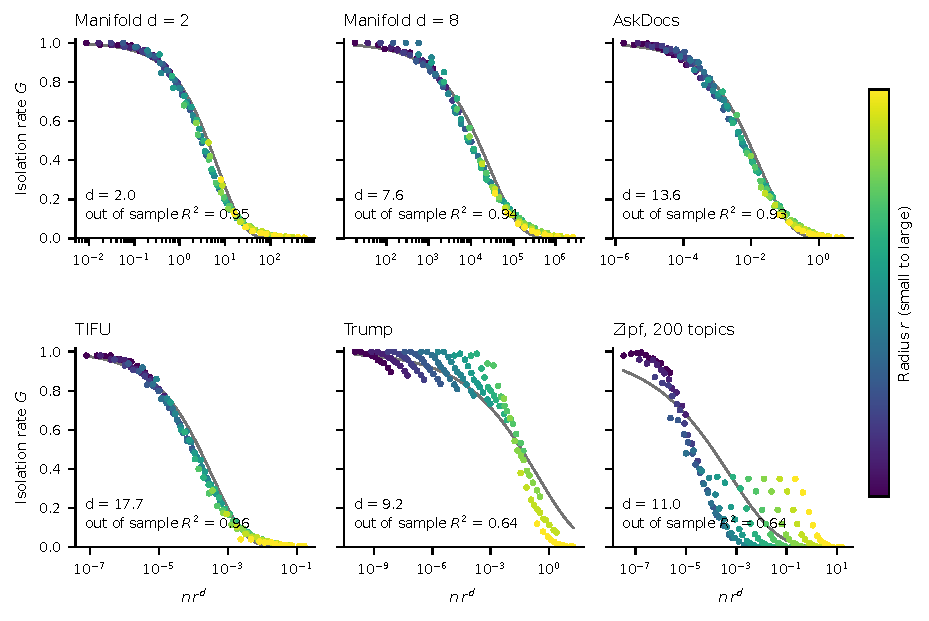
\includegraphics[width=\textwidth]{figures/collapse.pdf}
\caption{Isolation rate $G$ against $n r^{d}$ on a log scale, one panel per corpus, colour by radius $r$. Points from different radii fall on one curve where the law holds (AskDocs, TIFU, the manifolds) and separate where it fails (Trump, the Zipf mixture).}
\label{fig:collapse}
\end{figure*}

\subsection{Where the collapse fails, and why}

Trump and the Zipf mixture fail the fit (out of sample $R^2$ 0.64 for both, and 0.56 with sd 0.09 for Trump across seeds). In a 5{,}000-document sample of Trump, 3.4\% of documents have a near duplicate within cosine distance 0.02, against 0.0\% in AskDocs and TIFU, and the TwoNN dimension of its twenty $k$-means clusters runs from 2.0 to 16.2 (coefficient of variation 0.52, against 0.15 for AskDocs and 0.10 for TIFU). The clusters of dimension near 2 are slogans and the clusters near 16 are discussion. Removing the 266 near duplicates leaves the out of sample $R^2$ at 0.74, so the cause is the spread of local dimension and one global $d$ cannot describe both kinds of cluster. The Zipf mixture fails for the related reason of unequal topic mass, with no duplicates. The $R^2$ of the collapse fit is therefore a diagnostic: a corpus that collapses has one dimension and one sample size formula, and a corpus that does not needs a mixture.

\subsection{The finite population correction}

Table~\ref{tab:fpc} compares $G$ and $G\,(1 - n/N)$ with the true missing mass $M$ of the finite corpus over four corpora (AskDocs, Trump, TIFU and the Zipf mixture), six sample sizes from 100 to 5{,}000 and six radii, 144 cells. Uncorrected, $G$ has a mean absolute error of 0.068 and a maximum of 0.42, reached at $n = 5{,}000$ of $N = 10{,}000$, where $G$ is twice $M$. Corrected, the mean error is 0.015, the maximum 0.11 and the Spearman correlation 0.996. Across the three seeds on the forum corpora the corrected error is 0.010 on AskDocs, 0.013 on TIFU and 0.009 on Trump, so the correction holds on the corpus that fails the collapse as well.

\begin{table}[t]
\centering
\small
\begin{tabular}{rrrr}
\toprule
$n$ & $M$ (true) & $G$ & $G\,(1 - n/N)$ \\
\midrule
100 & 0.729 & 0.749 & 0.743 \\
200 & 0.665 & 0.684 & 0.672 \\
500 & 0.565 & 0.600 & 0.574 \\
1{,}000 & 0.479 & 0.534 & 0.486 \\
2{,}000 & 0.378 & 0.463 & 0.380 \\
5{,}000 & 0.211 & 0.384 & 0.212 \\
\bottomrule
\end{tabular}
\caption{Missing mass of the finite corpus, mean over four corpora and six radii at each $n$. $N$ is 10{,}000 for the three forum corpora and 20{,}000 for the Zipf mixture.}
\label{tab:fpc}
\end{table}

\subsection{Theme coverage is a question about a partition}
\label{sec:themes}

With thirty themes per corpus, the share of theme mass present in a sample is the same in all eight forum and census corpora at every $n$: 0.58 to 0.65 at $n = 25$, 0.82 to 0.86 at $n = 50$, 0.94 to 0.98 at $n = 100$ and 0.99 to 1.00 at $n = 200$ (Figure~\ref{fig:themes}). Equation~\ref{eq:gt}, evaluated on each corpus's theme masses, reproduces these values with a mean absolute error of 0.005. Over the same samples, coverage at a fixed resolution ($1 - G$ at $r = 0.34$) runs from 0.003 on AskDocs to 0.77 on citizens at $n = 25$. A quantity that is the same everywhere cannot be ordered by one that differs tenfold, and the Spearman correlation across corpora between the two is accordingly near zero at every $n$.

The language model's enumeration behaves as the partition says it should. Within each corpus the mass of themes Gemma~4 reports present rises with $n$ along the label coverage curve (Spearman $+1.00$ in seven corpora and $+0.90$ in TIFU), and its precision against the label truth rises from 0.73 at $n = 25$ to 0.98 at $n = 400$. Merging the eight inventories into one shared taxonomy at four merge radii (42 to 187 shared themes) opens up differences across corpora, and those differences are predicted by the shared masses through Equation~\ref{eq:gt} (Spearman $+0.93$ to $+1.00$) and not by $G$ at any fixed radius ($+0.31$, $+0.21$, $+0.38$ and $-0.40$ at $n = 50$ for the four merges). Appendix~\ref{app:shared} gives the full table.

The two questions are therefore different functionals of the same geometry. Coverage of a partition is set by the partition's mass vector. The missing mass at resolution $r$ is set by the local geometry at scale $r$, and the two coincide only when the partition's cells are balls of radius $r$, which thematic clusters are not. A user who asks ``have I seen every theme'' should use Equation~\ref{eq:gt} with the theme masses, which a pilot inventory supplies. A user who asks ``is every document within $r$ of something I have read'' should use $G$, the collapse law and Equation~\ref{eq:nstar}.

\begin{figure}[t]
\centering
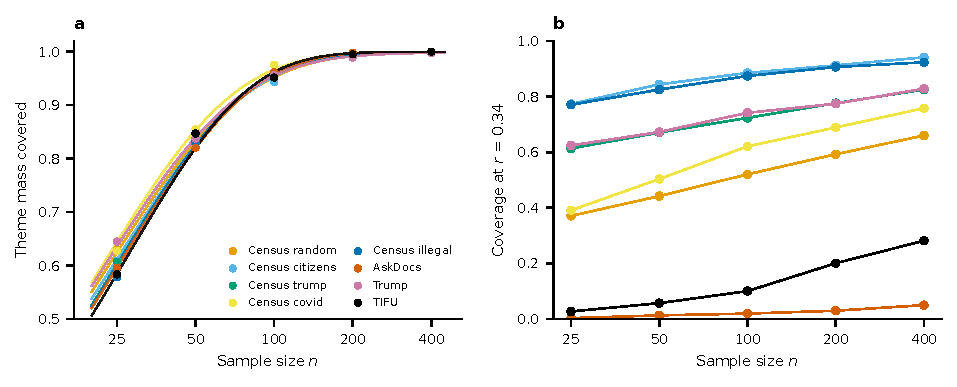
\includegraphics[width=\columnwidth]{figures/themes.pdf}
\caption{Share of theme mass present in a sample against $n$, eight corpora with thirty themes each (points), and the Good-Turing expectation of Equation~\ref{eq:gt} from each corpus's theme masses (lines).}
\label{fig:themes}
\end{figure}

\subsection{Truth Social and Bluesky}

\textcolor{red}{[Pending: the two 50{,}000-post samples are being embedded. This subsection will report their $d$, collapse $R^2$ and finite population correction once the run lands.]}

\section{Discussion}

The procedure a user follows has four steps. Choose the resolution $r$ that matches the question: a coarse $r$ for ``are the main kinds of post represented'', a fine $r$ for ``has every specific claim been seen''. Embed a pilot of about 2{,}000 documents and estimate $d$ by TwoNN. Fit Equation~\ref{eq:collapse} on nested subsamples of the pilot and check its $R^2$. Read $n^{*}$ from Equation~\ref{eq:nstar} and, after the sample is drawn, report $G\,(1 - n/N)$ as the share of the corpus the sample leaves uncovered. No step needs labels, and the whole runs on a laptop once the embeddings exist.

The survey analogy is exact in two places and instructive in a third. The finite population correction is the same factor for the same reason. The dimension $d$ plays the role of the variance: it is the one property of the population that the sample size formula needs, and like the variance it is estimated from a pilot. The third place is the margin of error. A survey's margin bounds the error of a proportion, and a corpus sample's plain mean already does that job well, to within 0.01 for cluster proportions at $n = 1{,}000$ in our data. The missing mass bounds something else, the mass of content the sample has no example of, which is the error that matters for enumeration: listing the themes, finding the rare claim, checking that a summary had the chance to mention something. The two margins answer different questions, and a report of a corpus sample should carry both.

The theme result explains two failures that an applied reader will have met. A free summary written from a sample is stable across draws at a rate that depends on the summarizer's own granularity, and a theme inventory of fixed size covers at the same rate in every corpus. Both readouts are relative to the corpus, and both are blind to how broad the corpus is at any absolute scale. The breadth that the sample size formula is about lives at a resolution, and only a readout at that resolution can see it.

The collapse diagnostic has a use beyond the formula. A corpus whose isolation surface does not collapse is one where slogans and discussion, or several registers, sit at different scales, and a single sample size will oversample one and undersample the other. The probe of local dimension across clusters locates the registers, and a stratified sample with a size per stratum is the natural next step.

\section*{Limitations}

The resolution $r$ is a cosine distance in the space of one encoder. The law held under both encoders on AskDocs and TIFU, but $d$ changed with the encoder, from 13.6 under Qwen3 to 18.3 under GTR on TIFU. A user must therefore fix the encoder before choosing $r$, and report the two together. Within one encoder, the same $r$ also means different things in different corpora (Section~\ref{sec:rcal}). Our calibration of $r$ rests on the judgments of two large language models, which agree with $\kappa = 0.55$ and place the crossing at different distances, and no person checked them.

The required sample grows as $r^{-d}$, so the formula is useful only at resolutions where the required sample is a feasible number. At $d = 15$, halving $r$ multiplies the required sample by about 33{,}000. The formula helps plan a sample at the resolution of the question, and it cannot make a fine resolution affordable.

The constants $a$ and $b$ must be fitted for each corpus. We can explain why $b$ is below 1, but we have no expression that predicts its value.

The pilot threshold of 0.95, and the gap of a quarter between the two estimates of $d$, were both chosen on the corpora of this paper. The band of two thirds to one and a half times $n^{*}$ is empirical, and resampling the pilot does not reproduce it. The corpora are English social media and forum text, and the Truth Social and Bluesky collections are political collections, so their values of $d$ describe those collections.

The unit of sampling is the document. Posts by the same account are correlated, and a design that samples accounts would need a version of the estimator for clusters.


\bibliography{references}

\appendix
\section{Synthetic smoke test}
\label{app:smoke}

The Zipf topic mixtures have 20{,}000 documents in 64 dimensions. Four settings vary the number of topics (50, 200 or 500), the Zipf exponent and the noise. Each setting was run at three seeds and eleven sample sizes from 50 to 5{,}000. Table~\ref{tab:smoke} compares coverage $1 - G$ with the true topic mass coverage at radius $\alpha$ times the median pairwise distance of a pilot.

\begin{table}[h]
\centering
\small
\begin{tabular}{rrr}
\toprule
$\alpha$ & Spearman $\rho$ & mean absolute error \\
\midrule
0.5 & 0.968 & 0.029 \\
0.4 & 0.797 & 0.091 \\
0.3 & 0.677 & 0.209 \\
0.2 & 0.576 & 0.521 \\
0.1 & 0.307 & 0.869 \\
\bottomrule
\end{tabular}
\caption{Agreement of $1 - G$ with true topic coverage on the Zipf mixtures, 132 samples.}
\label{tab:smoke}
\end{table}

\section{The sample size formula by corpus}
\label{app:nstar}

Equation~\ref{eq:collapse} was fitted on cells with $n \le 1{,}000$, five draws per cell. Equation~\ref{eq:nstar} then gave $n^{*}$ for $\varepsilon \in \{0.3, 0.2, 0.1\}$ at every radius where the mean surface crosses $\varepsilon$ at some $n > 1{,}000$, and the crossing was interpolated on the log scale between grid points. Table~\ref{tab:nstar} reports the ratio of predicted to empirical sample size. The grid steps by a factor of about 1.5 between adjacent sample sizes, and the interpolated crossing varies across the five draws by a median of 6\%. Leaving out the Zipf mixture, 10 of the 18 cases on failing text pairs fall within a factor of 1.5 and 14 within 2. With $a$ and $b$ fitted on nested subsamples of one 2{,}000-document pilot instead of draws from the whole corpus, 76 of the 83 cases on passing pairs fall within 1.5 and 81 within 2.

\begin{table}[h]
\centering
\small
\begin{tabular}{llrrrr}
\toprule
Corpus & Enc. & cases & median & $\le 1.5$ & $\le 2$ \\
\midrule
AskDocs & Qwen3 & 5 & 1.04 & 5 & 5 \\
Truth Social & Qwen3 & 6 & 0.88 & 5 & 6 \\
Census random & Qwen3 & 3 & 0.81 & 2 & 2 \\
Manifold $d{=}2$ & none & 9 & 1.15 & 9 & 9 \\
TIFU & Qwen3 & 6 & 1.08 & 6 & 6 \\
Bluesky & Qwen3 & 5 & 0.74 & 3 & 4 \\
TIFU & GTR & 17 & 1.24 & 17 & 17 \\
Manifold $d{=}8$ & none & 7 & 1.12 & 7 & 7 \\
AskDocs & GTR & 16 & 0.96 & 14 & 16 \\
Manifold $d{=}4$ & none & 9 & 1.09 & 9 & 9 \\
\midrule
Census illegal & Qwen3 & 3 & 1.24 & 2 & 3 \\
Census covid & Qwen3 & 3 & 1.22 & 3 & 3 \\
Trump & Qwen3 & 2 & 1.14 & 2 & 2 \\
Census trump & Qwen3 & 2 & 1.56 & 1 & 2 \\
Census citizens & Qwen3 & 2 & 2.06 & 0 & 1 \\
Trump & GTR & 6 & 1.86 & 2 & 3 \\
Zipf, 200 topics & none & 5 & 69 & 0 & 0 \\
\bottomrule
\end{tabular}
\caption{Predicted over empirical sample size for a target isolation rate, in the order of Table~\ref{tab:collapse}. GTR rows pool three samples of the forum corpus.}
\label{tab:nstar}
\end{table}

\section{Coverage of a theme inventory}
\label{app:themes}

Each of the eight forum and census corpora received inventories of themes by $k$-means on the full Qwen3 embeddings at $K = 10$, 30 and 100, and two inventories with skewed masses at $K = 30$: one from $k$-means++ seeding without refinement, one by merging the 100 clusters into 30 groups of Zipf sizes. The effective number of themes (the exponential of the entropy of the masses) ranges from 6.8 to 91. For each inventory and the 1{,}200 samples of Section~\ref{app:summaries}, Table~\ref{tab:themes} gives the range across corpora of the share of theme mass present. The expected coverage $\sum_k m_k (1 - (1 - m_k)^{n})$ matches the observed value to a mean absolute error of 0.004 over all cells. For the $K = 30$ inventory, Gemma~4 \citep{gemma4} was shown each sample and the list of named themes and asked which were present, with a supporting document for each. The mass of themes it reported rose with $n$ along the label coverage curve in every corpus, and the share of its reports that the labels confirm rose from 0.73 at $n = 25$ to 0.98 at $n = 400$.

\begin{table}[h]
\centering
\small
\begin{tabular}{lccc}
\toprule
Inventory & $n{=}25$ & $n{=}50$ & $n{=}100$ \\
\midrule
$k$-means, $K{=}10$ & 0.89 to 0.94 & 0.98 to 1.00 & 1.00 \\
$k$-means, $K{=}30$ & 0.58 to 0.64 & 0.82 to 0.85 & 0.94 to 0.98 \\
$k$-means, $K{=}100$ & 0.25 to 0.30 & 0.44 to 0.48 & 0.67 to 0.72 \\
seeding only, $K{=}30$ & 0.60 to 0.72 & 0.82 to 0.88 & 0.94 to 0.96 \\
Zipf merge, $K{=}30$ & 0.79 to 0.84 & 0.87 to 0.91 & 0.93 to 0.96 \\
\bottomrule
\end{tabular}
\caption{Share of theme mass present in a sample, range across eight corpora.}
\label{tab:themes}
\end{table}

\begin{figure}[h]
\centering
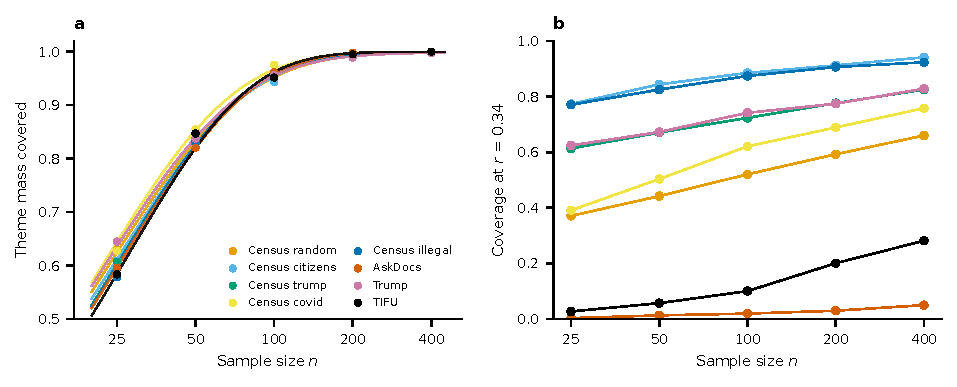
\includegraphics[width=\columnwidth]{figures/themes.pdf}
\caption{(a) Share of theme mass present in a sample against $n$ for the $K = 30$ inventory, eight corpora (points), with the expected coverage from each corpus's masses (lines). (b) Coverage $1 - G$ at the fixed radius $r = 0.34$ for the same samples.}
\label{fig:themes}
\end{figure}

\section{Summary stability}
\label{app:summaries}

For each of the eight forum and census corpora and each $n \in \{25, 50, 100, 200, 400\}$, thirty independent samples were summarized by Gemma~4 at temperature 0 in one paragraph of at most 150 words, and the summaries were embedded with Qwen3-Embedding-8B. Instability is the mean pairwise cosine distance among the thirty summaries. Within every corpus instability falls with $n$ and tracks $G$ (Spearman $+0.40$ to $+1.00$, seven of eight at $+0.70$ or above). Across corpora at a fixed $n$, Spearman of instability with $G$ is $+0.14$, $+0.12$, $+0.12$, $+0.07$ and $-0.17$ at $n = 25$ to 400, with bootstrap bands that include zero. TIFU illustrates why: its $G$ is near 1 at the shared radius and its summaries are the most stable, because the model summarizes it as stories of mishap whichever thirty stories it is given.

\section{A bound for functions that are stable at scale $r$}
\label{app:bound}

For a document function $f$ with range 1 that takes the same value on documents within $r$ of each other, the estimate of the corpus mean of $f$ formed by giving each corpus document the value of its nearest sampled document errs by at most $v(r) + M(r)$, where $v(r)$ is the share of covered documents whose nearest sampled document disagrees with them on $f$. On fifty cluster indicator functions over four corpora, six sample sizes and six radii, the bound held in 144 of 144 cells and was loose for proportions (median 22 times the realised error), where the plain sample mean already errs by 0.003 to 0.07.

\section{Prompts}
\label{app:prompts}

\paragraph{Summary.} ``Below are $\{n\}$ documents sampled from a larger collection. Write a summary of the collection in one paragraph of at most 150 words. Cover the main themes in proportion to how often they appear, name notable minority themes briefly, and do not mention individual document numbers.''

\paragraph{Theme naming.} ``The $\{m\}$ documents below were grouped together because they are about the same theme. Give the theme a short name (at most 8 words) and a one-sentence definition that would let a reader decide whether a new document belongs to it. Answer as JSON with keys name and definition.''

\paragraph{Enumeration.} ``Below are $\{n\}$ documents sampled from a larger collection, followed by a list of $\{K\}$ themes found in the full collection. Decide which themes are present among these $\{n\}$ documents. A theme is present only if you can point to one document that is primarily about it; in a small sample most themes will be absent, and similar-sounding themes are distinct, so pick the single best theme for each document. Answer with one line per present theme in the form theme\_id: document\_number.''

\paragraph{Same content.} ``Two documents from the same collection are shown. Judge their relation. SAME: they are about the same specific content (the same claim, question, event or story), so a reader who has read one would learn little new from the other. TOPIC: they are about the same general topic but different specific content. UNRELATED: they are about different topics.''


\end{document}
